%% BioMed_Central_Tex_Template_v1.06
%%                                      %
%  bmc_article.tex            ver: 1.06 %
%                                       %

%%IMPORTANT: do not delete the first line of this template
%%It must be present to enable the BMC Submission system to 
%%recognise this template!!

%%%%%%%%%%%%%%%%%%%%%%%%%%%%%%%%%%%%%%%%%
%%                                     %%
%%  LaTeX template for BioMed Central  %%
%%     journal article submissions     %%
%%                                     %%
%%         <14 August 2007>            %%
%%                                     %%
%%                                     %%
%% Uses:                               %%
%% cite.sty, url.sty, bmc_article.cls  %%
%% ifthen.sty. multicol.sty		   %%
%%				      	   %%
%%                                     %%
%%%%%%%%%%%%%%%%%%%%%%%%%%%%%%%%%%%%%%%%%


%%%%%%%%%%%%%%%%%%%%%%%%%%%%%%%%%%%%%%%%%%%%%%%%%%%%%%%%%%%%%%%%%%%%%
%%                                                                 %%	
%% For instructions on how to fill out this Tex template           %%
%% document please refer to Readme.pdf and the instructions for    %%
%% authors page on the biomed central website                      %%
%% http://www.biomedcentral.com/info/authors/                      %%
%%                                                                 %%
%% Please do not use \input{...} to include other tex files.       %%
%% Submit your LaTeX manuscript as one .tex document.              %%
%%                                                                 %%
%% All additional figures and files should be attached             %%
%% separately and not embedded in the \TeX\ document itself.       %%
%%                                                                 %%
%% BioMed Central currently use the MikTex distribution of         %%
%% TeX for Windows) of TeX and LaTeX.  This is available from      %%
%% http://www.miktex.org                                           %%
%%                                                                 %%
%%%%%%%%%%%%%%%%%%%%%%%%%%%%%%%%%%%%%%%%%%%%%%%%%%%%%%%%%%%%%%%%%%%%%


\NeedsTeXFormat{LaTeX2e}[1995/12/01]
\documentclass[10pt]{bmc_article}    



% Load packages
\usepackage{cite} % Make references as [1-4], not [1,2,3,4]
\usepackage{url}  % Formatting web addresses  
\usepackage{ifthen}  % Conditional 
\usepackage{multicol}   %Columns
\usepackage[utf8]{inputenc} %unicode support
\usepackage{graphicx}

%\usepackage[applemac]{inputenc} %applemac support if unicode package fails
%\usepackage[latin1]{inputenc} %UNIX support if unicode package fails
\urlstyle{rm}
 
 
%%%%%%%%%%%%%%%%%%%%%%%%%%%%%%%%%%%%%%%%%%%%%%%%%	
%%                                             %%
%%  If you wish to display your graphics for   %%
%%  your own use using includegraphic or       %%
%%  includegraphics, then comment out the      %%
%%  following two lines of code.               %%   
%%  NB: These line *must* be included when     %%
%%  submitting to BMC.                         %% 
%%  All figure files must be submitted as      %%
%%  separate graphics through the BMC          %%
%%  submission process, not included in the    %% 
%%  submitted article.                         %% 
%%                                             %%
%%%%%%%%%%%%%%%%%%%%%%%%%%%%%%%%%%%%%%%%%%%%%%%%%                     


%%\def\includegraphic{}
%%\def\includegraphics{}



\setlength{\topmargin}{0.0cm}
\setlength{\textheight}{21.5cm}
\setlength{\oddsidemargin}{0cm} 
\setlength{\textwidth}{16.5cm}
\setlength{\columnsep}{0.6cm}

\newboolean{publ}

%%%%%%%%%%%%%%%%%%%%%%%%%%%%%%%%%%%%%%%%%%%%%%%%%%
%%                                              %%
%% You may change the following style settings  %%
%% Should you wish to format your article       %%
%% in a publication style for printing out and  %%
%% sharing with colleagues, but ensure that     %%
%% before submitting to BMC that the style is   %%
%% returned to the Review style setting.        %%
%%                                              %%
%%%%%%%%%%%%%%%%%%%%%%%%%%%%%%%%%%%%%%%%%%%%%%%%%%
 

%Review style settings
\newenvironment{bmcformat}{\begin{raggedright}\baselineskip20pt\sloppy\setboolean{publ}{false}}{\end{raggedright}\baselineskip20pt\sloppy}

%Publication style settings
%\newenvironment{bmcformat}{\fussy\setboolean{publ}{true}}{\fussy}



% Begin ...
\begin{document}
\begin{bmcformat}


%%%%%%%%%%%%%%%%%%%%%%%%%%%%%%%%%%%%%%%%%%%%%%
%%                                          %%
%% Enter the title of your article here     %%
%%                                          %%
%%%%%%%%%%%%%%%%%%%%%%%%%%%%%%%%%%%%%%%%%%%%%%

\title{Building blocks for automated elucidation of metabolites: Prediction of mass spectra}
 
%%%%%%%%%%%%%%%%%%%%%%%%%%%%%%%%%%%%%%%%%%%%%%
%%                                          %%
%% Enter the authors here                   %%
%%                                          %%
%% Ensure \and is entered between all but   %%
%% the last two authors. This will be       %%
%% replaced by a comma in the final article %%
%%                                          %%
%% Ensure there are no trailing spaces at   %% 
%% the ends of the lines                    %%     	
%%                                          %%
%%%%%%%%%%%%%%%%%%%%%%%%%%%%%%%%%%%%%%%%%%%%%%


\author{Miguel Rojas Cherto$^1$%
       \email{Miguel Rojas Cherto - m.rojas@lacdr.leidenuniv.nl}%
      \and
         Egon L Willighagen$^2$%
         \email{Egon L Willighagen - egon.willighagen@gmail.com}
       and 
         Christoph Steinbeck\correspondingauthor$^3$%
         \email{Christoph Steinbeck - steinbeck@ebi.ac.uk}%
      }
      

%%%%%%%%%%%%%%%%%%%%%%%%%%%%%%%%%%%%%%%%%%%%%%
%%                                          %%
%% Enter the authors' addresses here        %%
%%                                          %%
%%%%%%%%%%%%%%%%%%%%%%%%%%%%%%%%%%%%%%%%%%%%%%

\address{%
    \iid(1)Analytical Sciences Department, Leiden University, Leiden, The Netherlands\\
    \iid(2)Biomedical Center, Uppsala University, Uppsala, Sweden\\
    \iid(3)European Bioinformatics Center (EBI), Wellcome Trust Genome Campus, Hinxton, Cambridge, UK
}%

\maketitle

%%%%%%%%%%%%%%%%%%%%%%%%%%%%%%%%%%%%%%%%%%%%%%
%%                                          %%
%% The Abstract begins here                 %%
%%                                          %%
%% The Section headings here are those for  %%
%% a Research article submitted to a        %%
%% BMC-Series journal.                      %%  
%%                                          %%
%% If your article is not of this type,     %%
%% then refer to the Instructions for       %%
%% authors on http://www.biomedcentral.com  %%
%% and change the section headings          %%
%% accordingly.                             %%   
%%                                          %%
%%%%%%%%%%%%%%%%%%%%%%%%%%%%%%%%%%%%%%%%%%%%%%


\begin{abstract}
        % Do not use inserted blank lines (ie \\) until main body of text.
        \paragraph*{Background:} The majority of metabolites in organisms from the various kingdoms of life is still unknown \cite{Dunn:2005p2594}, with
increseasing severness from mammals via microbes, fungi and plants. Computer-assisted structure elucidation \cite{steinbeck2001, steinbeck2003} can be employed to decipher the structure of unknown metabolites based on spectroscopic evidence. 
      
        \paragraph*{Results:} Here we report on our recent development of MEDEA, an algorithmic framework for the prediction of mass spectra for a given chemical structure. MEDEA recursively apply a set of fragmentation rules to a chemical graph until no further fragmentation can be applied. The result of this procedure is a predicted mass spectrum without intensities. MEDEA then estimated the probability for each fragmentation based on a decision tree algorithm and a description of the reaction center based on QSPR descriptors. The algorithmic and visual framework for this work have been developed as part of Bioclipse \cite{}.

        \paragraph*{Conclusions:} A combination of mass spectra predicted by MEDEA with other spectral and chromatographic information, combined with further evidence
such as genetic capability of an organism to perform certain biochemical reactions will open up the path to a framework for the identification of unknown metabolites. 

        \paragraph*{Availabily:} MEDEA is available as a Bioclipse feature. It is open source and can be used, modified and redistributed under Gnu General Public License (GPL).  
\end{abstract}



\ifthenelse{\boolean{publ}}{\begin{multicols}{2}}{}




%%%%%%%%%%%%%%%%%%%%%%%%%%%%%%%%%%%%%%%%%%%%%%
%%                                          %%
%% The Main Body begins here                %%
%%                                          %%
%% The Section headings here are those for  %%
%% a Research article submitted to a        %%
%% BMC-Series journal.                      %%  
%%                                          %%
%% If your article is not of this type,     %%
%% then refer to the instructions for       %%
%% authors on:                              %%
%% http://www.biomedcentral.com/info/authors%%
%% and change the section headings          %%
%% accordingly.                             %% 
%%                                          %%
%% See the Results and Discussion section   %%
%% for details on how to create sub-sections%%
%%                                          %%
%% use \cite{...} to cite references        %%
%%  \cite{koon} and                         %%
%%  \cite{oreg,khar,zvai,xjon,schn,pond}    %%
%%  \nocite{smith,marg,hunn,advi,koha,mouse}%%
%%                                          %%
%%%%%%%%%%%%%%%%%%%%%%%%%%%%%%%%%%%%%%%%%%%%%%




%%%%%%%%%%%%%%%%
%% Background %%
%%
\section*{Background}

In the past two decades, research in biology has been shifting from a reductionist approach of 
studying smaller and smaller parts of organisms to a systems biology paradigm. On the analytical side 
we now study the behaviour of as many parts of the system as possible simultaneously in so-called "omics" 
approaches and on the synthetic side the parts studied earlier are integrated into dynamic biological networks
for the sake of simulation \cite{Weckwerth:2003p2788}.
In Metabolomics we study the changes in occurrence and concentration of as many metabolites as possible at once 
in an organism, organ or tissue or even a single cell \cite{MIZUNO:2008p2919}.  

XXX Talk about CASE here and MS and NMR with reference to our earlier work.

Considerable research work has been done for understanding the fundamental 
processes involved in the generation of a mass spectrum and, although the mechanisms of ion formation are still not 
completely understood, real advances have allowed changes in instrumentation. 
New methods of eliminating this irreproducibility are being 
studied\cite{bacon1984}.

The state of mass spectrometry at the beginning of the 21st century has recently been 
review by Lebedev and Zaikin \cite{Lebedev:2008p2704}

A detailed theoretical approximation can take into account the Ionization 
processes, the fragmentation reactions under consideration of thermodynamic and 
kinetic effects, statistic mechanic, quantum mechanic and molecular geometry. 
There is a fairly wide range of methods for the prediction of mass spectra.
   
The first and most recognized approximation for the fragmentation conduct was 
presented by the Quasi-equilibrium theory QET, originally formulated by 
Rosenstock et. al. (1952)\cite{mcLafferty1980}. Many of the actual ab-initio 
reaction prediction methods derive from it. The QE theory gives a physical 
description of mass-spectral behaviour. The derivation of the Potential 
Ionization follows the Franck-Condon process. On the other hand, the 
probability for the decomposition of an ion depends on its internal energy and 
its rate constant (K(E))functions. The K(E) was described by the 
Rice-Ramsperger-Kassel-Marcus\cite{marcus1952} (RRKM) theory (Robinson and 
Holbrook\cite{robinson1972,frost1973}). The main disadvantage of calculating 
the complete mass spectrum with the QET is the fact that it causes extremely 
high computational costs.

Due to the necessity of using methods which possess an acceptable precision and 
at the same time a rate (speed) of calculation, chemoinformatic have been 
developed parallel methods.

Thus, most of the methods used by chemoinformatics to predict mass spectra are 
forming part of CASE systems. The majority of structure elucidation methods 
using mass spectra to rank a proposed structure is based on mass spectra 
database search. They use data-mining techniques to find similar spectra and to 
assign hits, as for example MASSLIB\cite{massLib1987,henneberg1988} and 
SpecInf\cite{specInfo2007,bremser1988}. Other groups apply multivariate statistical 
analysis\cite{lohninger1987}, pattern recognition\cite{kwok1973,jalali2000} and artificial 
neural networks \cite{curry1990} of experimental mass spectra to classify 
substances. Nevertheless, none of them confronts with mass spectrometry 
behaviour.

The DENDRAL\cite{dendral1980} project, initiated 1965 and cited as the first Expert 
System (ES) developed in chemistry, attempted to simulate the mass spectra of 
candidate structures using a set of knowledge- or rule-based methods. It tried 
to resolve the problem of structure elucidation of organic compounds using mass 
spectral data. Yet, the DENDRAL project is considered rather an informational 
than a chemical part. It was posteriorly followed by Stirs\cite{haraki1981} system.

Other systems such as MASSIMO\cite{masssimo2003}, MASSIS\cite{massis2003a,massis2003b} and 
the latest work by Kerber A.\cite{kerber2006} (in chronological order) attempt to 
simulate a quantitative reaction model occurring  in a mass spectrometer . They 
are further steps in the simulation of mass-spectral behaviour without going 
across ab-initio terms.

MASSIMO, developed by Gasteiger and co-workers, applies reaction rules 
according to their probabilities to the target structure, thus obtaining the 
reaction-tree scheme. Afterwards this reaction-tree scheme is converted into a 
simulated mass spectrum. The reaction database providing the probabilities of 
reactions is generated with the help of another system, FRANZ (Fragmentation 
and Rearrangement ANalyZer). It extracts automatic knowledge about the 
reactions from a spectrum and the corresponding structure.

In MASSIS, the simulation is performed from a pivot knowledge database. The 
pivot database contains information about reaction rules, functional groups and 
small fragments. Once the net-reaction is obtained, the peak intensity is 
determined using the information from a prior fragment-relationship study also 
included in the database. Kerber extracts the simulation of mass spectra to 
rank structure candidates for the elucidation of structures using 
Computer-Assisted Structure Elucidation (CASE). The MASSIS and Kerber group are 
not able to calculate intensities of mass spectra, instead both systems compare 
the masses of the fragments to $m/z$ values of experimental spectra.


\subsection{The MEDEA System}

As indicated previously, this work is focused on the simulation of 70eV 
electron ionization (EI) mass spectrometry (MS). For quite some time now the EI 
MS has been accepted for containing more information and for the fact that it 
can be interpreted easily\footnote{It produces the formation of the simple 
loaded cations which are dissociated in uni-molecular reactions.}. The 
methodology followed by Gasteiger's group, modelling the events occurring in 
the mass spectrometer with the FRANZ-MASSIMO\cite{gasteiger1992} system, is the 
right approach for obtaining a well-predicted mass spectrum. But the problem is 
that Gasteiger's work is, of course as almost always, either obscurely 
explained or written in German. And furthermore, in many cases the origin of 
constants and variables is not fully described. That is why my work does not 
only copy his work but tries to reproduce, explain, compare and improve the 
algorithms and the methodologies followed by him.

This project is divided into three separated parts, namely the ionization 
potential acquisition, the learning process and the prediction process. All 
three parts are integrated in a system manly MEDEA which makes eases its 
handling. But, at the same time they work independently. As Gasteiger pointed 
out, \emph{we will be able to predict the mass spectrum of a given structure if 
we understand, know and model the fragmentation and rearrangement steps 
occurring in the mass spectrometer}. The most  important ionization, 
fragmentation and rearrangement rules have been known for a long time now 
\cite{mcLafferty1980,budzikewicz1967}. However, there is scant information about the 
reactivity of each of these reactions. If our system has the capacity to set 
reactivity to fragmentations, it will be able to simulate mass spectra of 
structures previously not analysed.


All three independent components of the MEDEA system, ionization potential 
acquisition, the learning process and the prediction process, are listed below, 
together with a brief description of each component.
 
\begin{enumerate} \item The first part tries to correlate a 
structure with its ionization potential energy. Therefore, the application of a 
decision tree was chosen as machine learning method. The structures are encoded 
in the database using different descriptors. The data for the training of the 
machine learning constitute a database comprising more than 3000 structures by 
their descriptors and their experimental ionization energy.

\item The second part of this work is dedicated to building a pivot database 
which derives the correlation between reactions and their reactivities. These 
informations are extracted from experimental mass spectra. The reactions are 
described by physicochemical effects of their reaction center. Each reaction 
type includes its own database.

\item The last part is essential for the user who is only 
interested in the prediction of the mass spectrum of an unknown analyte. The 
prediction of the reactivity for each fragmentation is deduced from a machine 
learning data processing from the previous pivot database.
\end{enumerate}

 
%%%%%%%%%%%%%%%%%%%%%%%%%%%%
%% Results and Discussion %%
%%
\section*{Results and Discussion}

MEDEA is able to predict mass spectral trees from a given molecular graph based on 
the recursive application of XXX rules for fragmentation and re-arrangement. 
    

%%%%%%%%%%%%%%%%%%%%%%
\section*{Conclusions}
  Text for this section \ldots


  
%%%%%%%%%%%%%%%%%%
\section*{Methods}
  \subsection*{Prediction of ionization potential}
    Text for this sub-section \ldots

  \subsection*{Generating fragmentation trees}
    Text for this sub-section \ldots

  \subsection*{Machine learning for the prediction of fragmentation probabilities}
 
\begin{figure}[htp]
\begin{center}
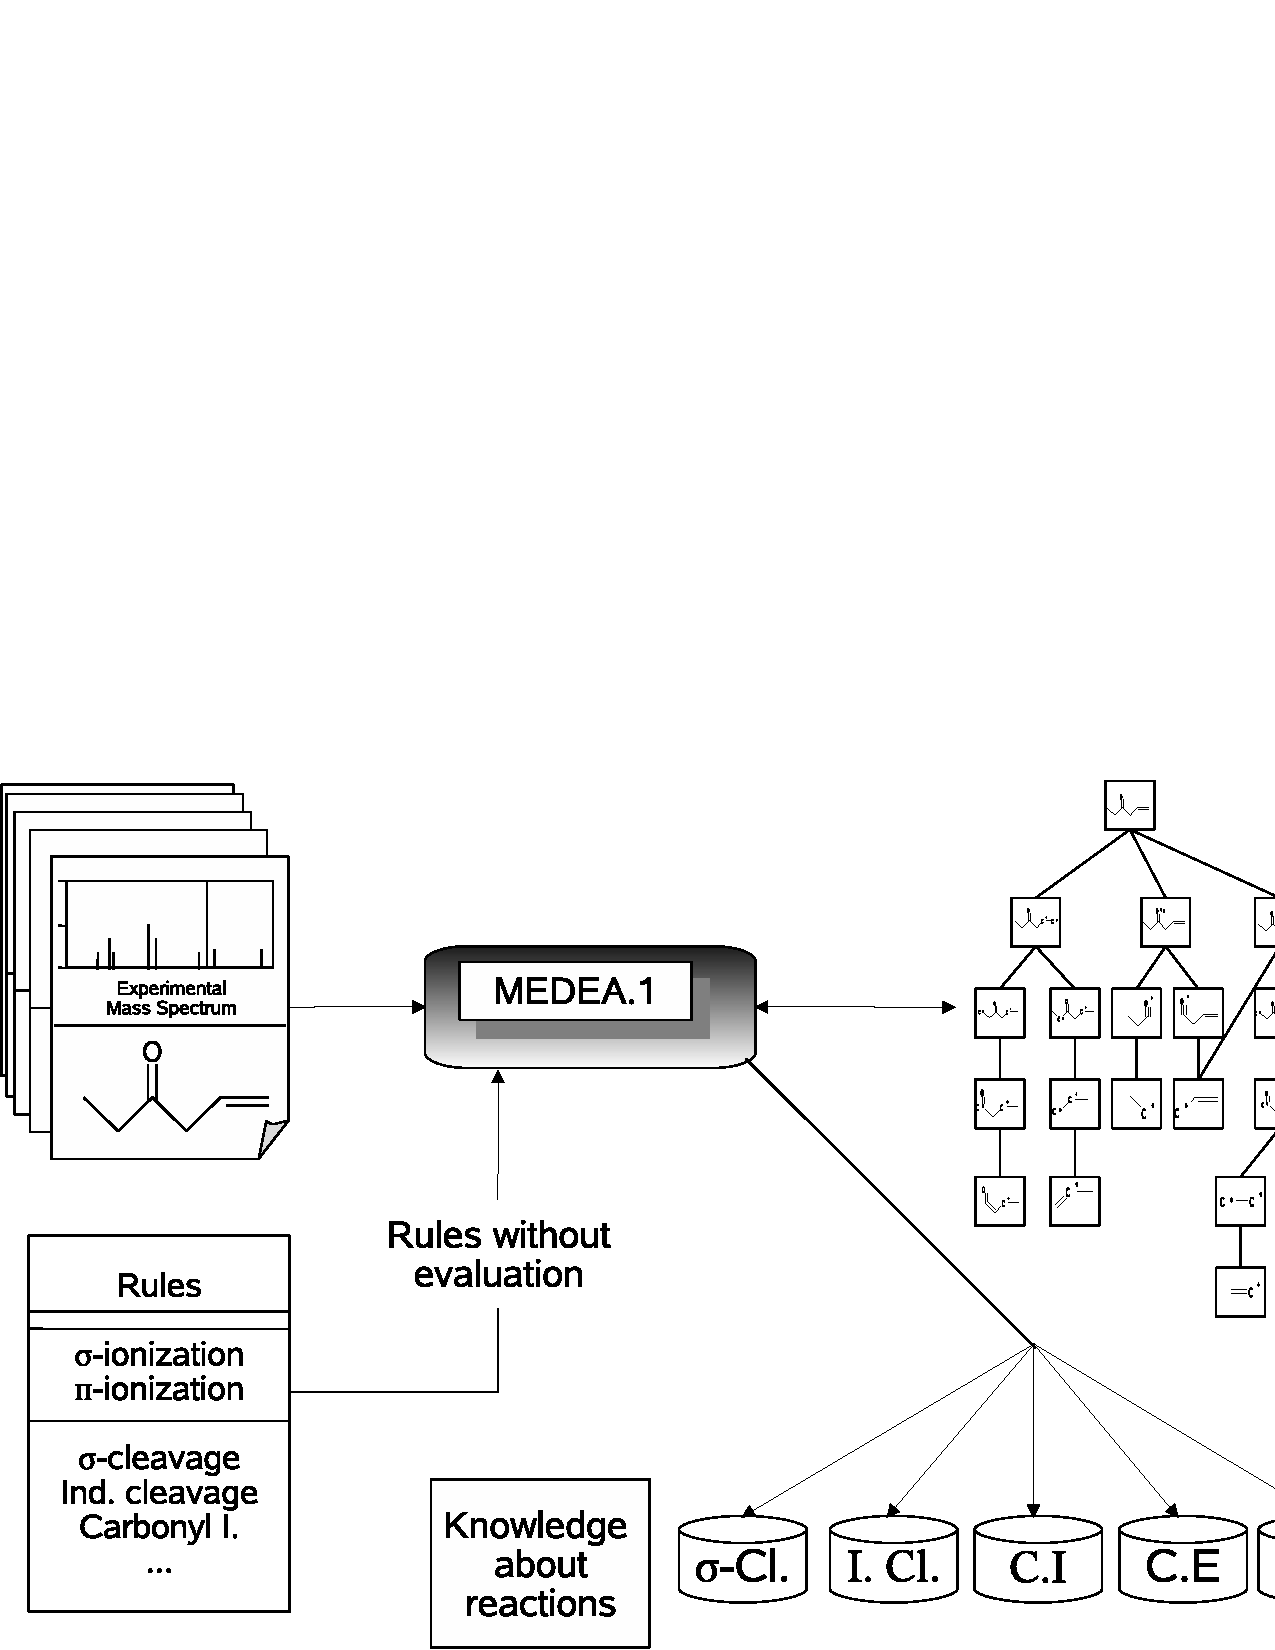
\includegraphics[scale=.5]{figures/learningProcessRepresentation.pdf} \caption[Mass 
spectra learning]{{\bf{Mass spectra learning}}. Process 1: Basic design of 
MEDEA system for extracting reaction knowledges.}
\label{fig:learningProcessRepresentation}
\end{center}
\end{figure}



\section{Introduction}

One of the interest in a chemical laboratory is the prediction of reactions and 
the knowledge of the factors influencing the success obtaining products. The 
easy way and first steps is the research literature. But evidently all 
experimental reactions were not analyzed yet. The other way is through 
chemometrics methods which extracts correlations from similar reactions. 
Analyzing mass spectrum fragmentations we confront with a even bigger problem. 
There is not any information about it and its experimental study is still 
difficult itself.

Thus, in this chapter aims how the inspection and the analysis the 
fragmentation and arrangement of reactions takes part in the mass spectrometer 
from a variety of chemical structures. An automatic method acquiring knowledges 
has been developed. It observes what reactions happen and what not. Once the 
network-reaction is obtained, the process extracts the probability for each 
fragmentation or arrangement reaction found and saves this information in a 
pivot-database which later will be used again. We can see the scheme of the 
process in the Figure \ref{fig:learningProcessRepresentation}. The cylinders 
represent the pivot database with the information about reaction knowledges.

\section{The Fragmentation Generator}

Important for managing automatically reaction is to have a fragmentation 
generator. The fragmentation generator follows carefully two goals:
\begin{enumerate}
\item The generator should be capable to reconstruct the decomposition 
reactions taking part on the mass spectrometer from a given chemical structure 
with the corresponding experimental mass spectrum, jointly with several 
predetermined fragmentation rules. Furthermore it should be also able to 
determine reaction probabilities of the obtained decomposition reactions.
\item It should file the evaluation of the reactions in separated blocs 
according the fragmentation processes from an abundant number of compound. This 
information date will be used later to provide with machine learning reactivity 
functions for each specific fragmentation process.
\end{enumerate}

\begin{figure}[htp]
\begin{center}
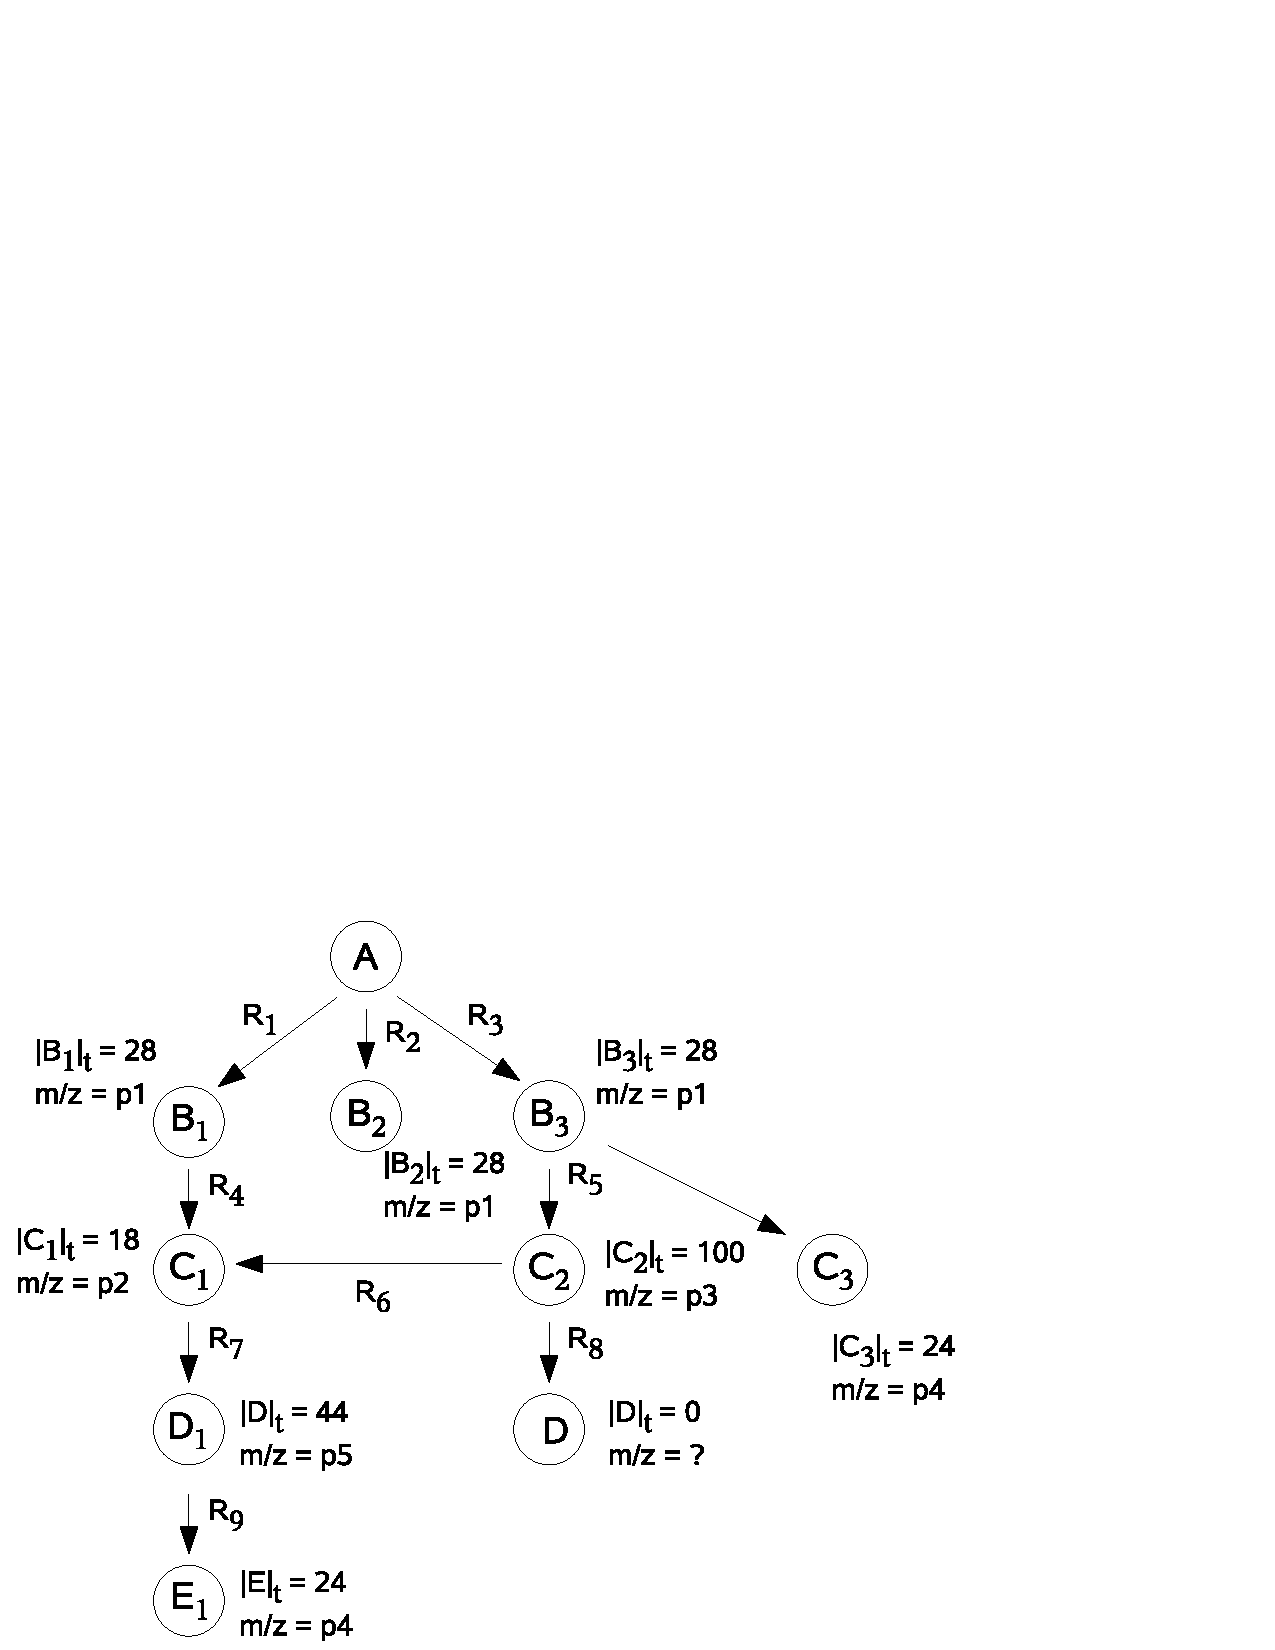
\includegraphics[scale=1.05]{figures/fragmentationGenerator2.pdf} 
\caption[Fragmentation generator scheme.]{{\bf{Fragmentation generator 
scheme.}}. First exercise: determination of the decomposition reaction in the 
mass spectrometer jointly with its evaluation. Second exercise: the previous 
process is repeated for a large number of compounds putting the evaluation of 
each fragmentation reaction in the corresponding database. Each reaction type 
has itself database.}
\end{center}
\label{fig:fragmenatationGenerator1}
\end{figure}

The Figure \ref{fig:fragmenatationGenerator1} shows the procedure to follow. 
Initially the process begins with the acquisition of chemical structures and 
their respective experimental spectrum, in my case the database come from the 
NIST database. Afterwards, the generator system generates a sequence of 
fragmentations and rearrangements, so-called decomposition-tree, using just 
specific reaction rules.

The reactions available and integrated in the generator are shown in Figure 
\ref{fig:reactionSetps}. They are reaction rules mechanized with CDK\cite{cdk2002} 
framework but they are not all reaction rules which CDK comtemplate. The rest 
of them will be added progressively according to the results.


\begin{figure}[htp]
\begin{center}
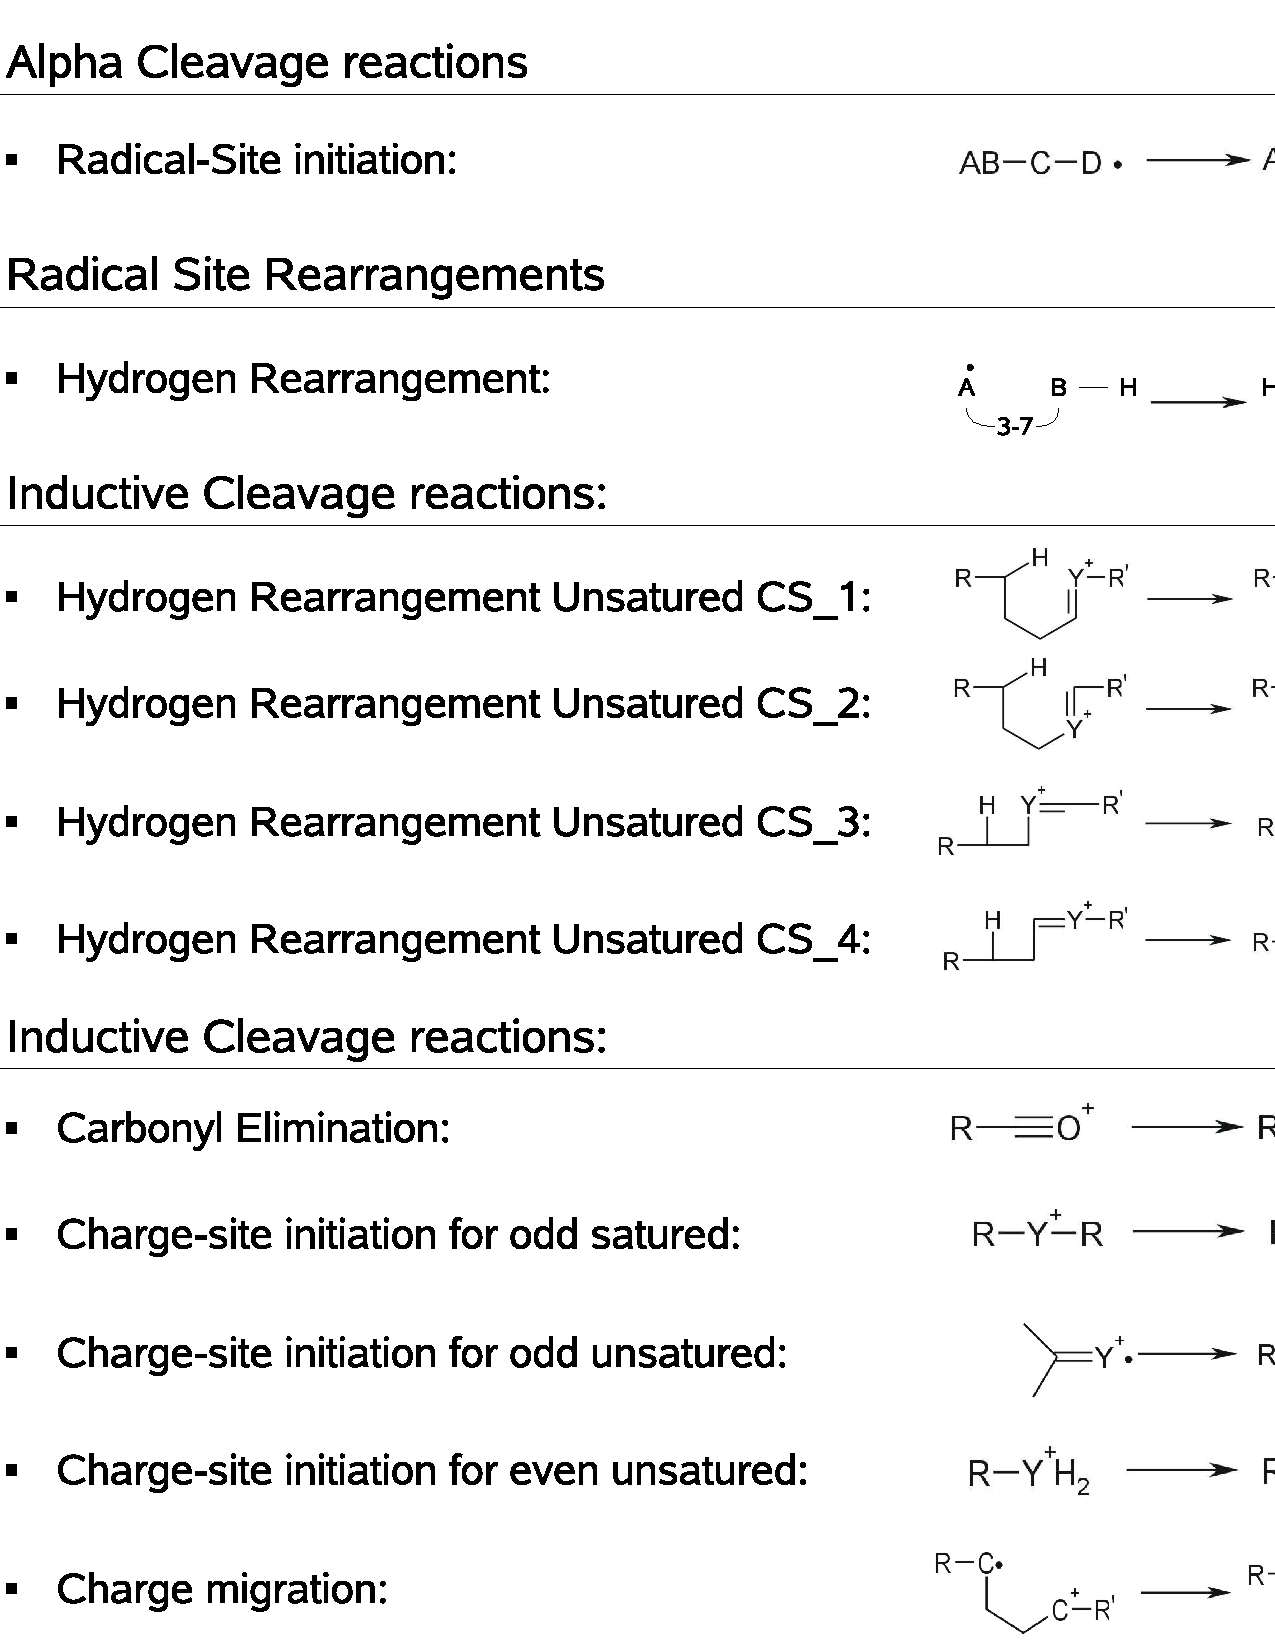
\includegraphics[scale=0.57]{figures/reactionTypes.pdf} 
\caption[Fragmentation rules.]{{\bf{Fragmentation rules.}}. Fragmentation rules 
which the fragmentation generator uses. In addition comes the Ionization 
reactions from lone pair electrons and $\pi$-bonds.}
\end{center}
\label{fig:reactionSetps}
\end{figure}

Once the process is finished the system obtains a network-reaction, shown in 
Figure \ref{fig:fragmenatationGenerator1} occupying the central position. The 
illustrated network-reaction reflects the fragments as boxes and the reactions 
as lines. As example, the reaction shown is a radical site initiation mechanism 
($\alpha$-cleavage) of an atom capsuling a single electron. It contains 
information about the reactant and the product, and the reaction probability. 
Consequently it is put in the $\alpha$-cleavage database.

This process is repeated for a lot of different structures which were 
previously selected according special features. So, using the fragmentation 
generator for more compounds it is possible to create a pivot-database 
containing information about a wide variety of reactions jointly with 
probability. The system collects in independent data according reaction types. 
Larger is the information collection much better will be the variety and 
preciser will be the prediction.

\section{Mode of Operation}

The obtaining of the network-reaction scheme and the determination of the 
probability for each fragmentation reaction from a chemical structure and its 
corresponding mass spectrum is divided in subsequent steps:

\begin{enumerate}
\item Checking the graphical structure of the compound.
\item Ionization evaluation process.
\item Extraction of the network-reaction tree.
\item Analysis of the network-reaction tree.
\item Storing evaluation fragmentation.
\end{enumerate}

\subsection{Structure Checking}

After the chemical structure and its spectrum are loaded the process starts 
with a compound's checking. The checking process inspects if the chemical 
structure has all features into agree. It just checks two features. One 
consists on checking if the hydrogens are explicit in the structure. In fact, 
in chemoinformatics is habitual to represent a structure with implicit 
hydrogens meaning that the structure does have hydrogens, it does not have 
initiated hydrogen as atom object but the atoms know how number of the 
hydrogens which are neighbour. Other side a structure can have explicit 
hydrogens und that means that hydrogen is such a atom object like C,  O or 
whatever. So, if the hydorgen are not explicit in the structure the checker 
uses the \emph{HydrogenAdder} method to add explicit hydrogens to satisfy 
valency. That is very important because the reaction rules in CDK can only 
yield correct results if they are explicit. We must think that some reactions 
are rearrangements of atoms which might be a hydrogen atom. Afterwards the 
system checks with the method \emph{LonePairElectronChecker} if each atom of 
the structure contains the correct number of lone pair electrons. If it doesn't 
have they are added.

\subsection{Ionization evaluation process \label{learningIP}}

Once the chemical structure was inspected containing all features correctly, 
the simulation can begin. The first step from the fragmentation generator is 
the ionization of the substance with the ionization rules before commented
as shown in figure XXX. In this case the ionizations are applied to lone pair electrons and 
$\pi$-systems, described on the previous section. Then, using a decission three 
methode the necessary energy is set. Finally, the probability of the ionization 
from the energy is extracted applying the Maxwell-Boltzmann statistics 
equation, Eq. \ref{eq:boltzannEq}.

Depending of the probability obtained to ionize the ions will be incorporated 
or not. The constraint limit to acquire those ions which have a probability 
higher than 0.10\%. Those ions with lower probability will be descanted.



\subsection{Extraction Reaction-Network}

Reaction-network groups all reactions and structures that might occur in the 
mass spectrometer by application of fragmentation generator. Additional to the 
fragmentation reactions shown in Figure \ref{fig:reactionSetps} are applied the 
ionization processes.

The reaction rules contained in fragmentation generator know only about the 
description of the reaction centre and the specification for generating the 
products.


The fragment contains information about its subsequent fragmentations and the 
previous fragments which have generated it.

In each new obtained product through the construction of the network-reaction 
must be generated all mesomers. Important is also making 
attention the formation of duplicates fragments ??. The method used to limit 
this error is with the \emph{Universalisomorphismus} method. A chemical 
fragment is analyzed once. If the fragment in question appears more time by the 
generation of the network-reaction is increased its counter. The counter is 
easily the number of time that this fragment appears.


Each new obtained fragment is analysed if it is shown in the experimental 
spectrum. If it is shown it is stored and fragmented again. If it is not shown 
the fragment is stored but it is not fragmented any more.


The process start with a structure and its respective experimental spectrum. 
The first process is the ionization. In the capitol X describes the process how 
is it calculated. The possible solutions are added in the ArrayList which is 
the responsible to handle the fragment to be analysed. Thus, the process starts 
with the possible ionization solutions. The ions solutions must be radical 
cation structures. For each ionized structure is applied the reaction rules 
specified before. Then, the system inspects if the products are a valid target 
to be saved. For this created restrictions. It inspects if the products are 
cations (only whose products that are cations are visualized in the mass 
spectrometer). Neutral and radical reactants generate never cations again. It 
inspects if the products are visualized in the spectrum, aa. That means if the 
molecular weight of the products are not visualized as a peak in the spectrum 
is expected that the reaction will produce. That is not fully correct. It is 
know that those whose reactions are not visualized in the spectrum, 
nevertheless might occur. Than, The system can not analyse these cases and they 
run away of the study. This can produce that  we loss information.

It inspects if the products were already previously obtained. The method used 
is the class Universalisomorphismus....

restrictions < 0.9 frequency.



Once the product gets through all restrictions, it is accepted, it is added to 
the arraylist for being again fragmented and rearranged. This loop is applied 
until the all fragments containing the arraylist are inspected.


This process has been applied for different structure-spectrum. Creating a 
pivot-database of reaction rules linked with reaction probabilities. Figure XXX shows the list containing the structures studied.

\section{Analysis of a Reaction-Network}


Once we have obtained the reaction-network which contains the information about 
all reaction occurring in the mass spectrometer for a specific chemical virtual 
structure, comes the extraction of the probabilities for each possible 
reaction. The next chapter explain the procedure and how the results are saved.

\subsection{Calculation of the Reaction Probability}

The reaction probabilities is calculated from the frequency of signal-peaks of 
the experimental spectrum. These experimental spectra were extracted from the 
NIST \cite{NIST2007} database and they were selected according to our opinion and 
experience by which they can produce the biggest variety of reactions. Another 
criterion was also that they should not contain more than altogether 40 peaks 
with a maximum representative.

FRANZ system, system which obtain probabilities from frequency peaks, studied 
different models to extract this information. Finally, they stated that the 
best algorithm given a reasonable results. The algoritm used, Equation 
\ref{ee}. is a reaction of first order and depends of kinetic approximation.

\begin{equation}
\label{ee}
P_i = 1-\left( \frac{\left |A \right 
|_t}{\left|A\right|_0}\right)^{-\frac{\textstyle B_{i}}{\textstyle k 
\sum_{k=1}^N B_{N}}}
\end{equation}

$P_{j}$ is the probability of the reaction from a compound $A$ (reactant) to a 
compound $B_{j}$ (product) in a specific time. $A_{0}$ is the concentration of 
the compound $A$ in time 0 and $A_{t}$ is the concentration of the compound $A$ 
in time t. $B_{i}$ is the concentration of the product which takes part in the 
reaction $i$ and $K$ are others products obtained from the compound $A$ and 
considered as neighbour compounds. And $k$ represents the symmetry. The 
symmetry is the number of time appearing the same reaction in the whole process.

The Sulz model I think it is the best model to simulate the probabilities. So 
the same algorithm has been implemented for me as well but with some changes 
due to same concepts which are to complicate to apply.

A problem with this probabilites extraction manner is that. Sulz implemented a 
new concept for escaping these problems, called lower and upper limit. They 
solute the uncertainly for the problematic cases. The lower and upper limit are 
extracted from heuristic methods and they increase or decrease the 
probabilities obtained from the Eq. In my system it was not implemented because 
they need too many rules and it had no time for the implementation. Otherwise, 
I added into the algorithm, Eq. X, that the concentration of each Substance 
will be re-calculated. That means that the concentration of the  child are not 
those frequency visualized but divided between the number of brothers. The 
example is represented for YY. Even though, this is not correct  the fragments 
with the same molecular weight have the same volume of quantity. They 
approximate the influence.


We have implemented, then that this symmetry contains information about the 
time. We think it should not have the same influence the same reaction but 
occurred in different times. There are cases with we must take into account.

\begin{equation}
\label{weightTotal}
P_i = 1-\left( \frac{\left |A \right 
|_t}{\left|A\right|_0}\right)^{-\frac{\textstyle B_{j}^*}{\textstyle 
\sum_{k=1}^N B_{N}^*}}
\end{equation}


\begin{center}
\begin{figure}[h]
\begin{enumerate}
\item more one fragment for a frequency peak
\item obtaining more than 1 products
\item the same product for different reactions
\item symmetry of reactions
\end{enumerate}
%\caption{Group of the organics compunds which have been divided to apply the
%training set}
\label{fig:listProbleCases}
\end{figure}
\end{center}


\begin{figure}[h]
 \begin{center}
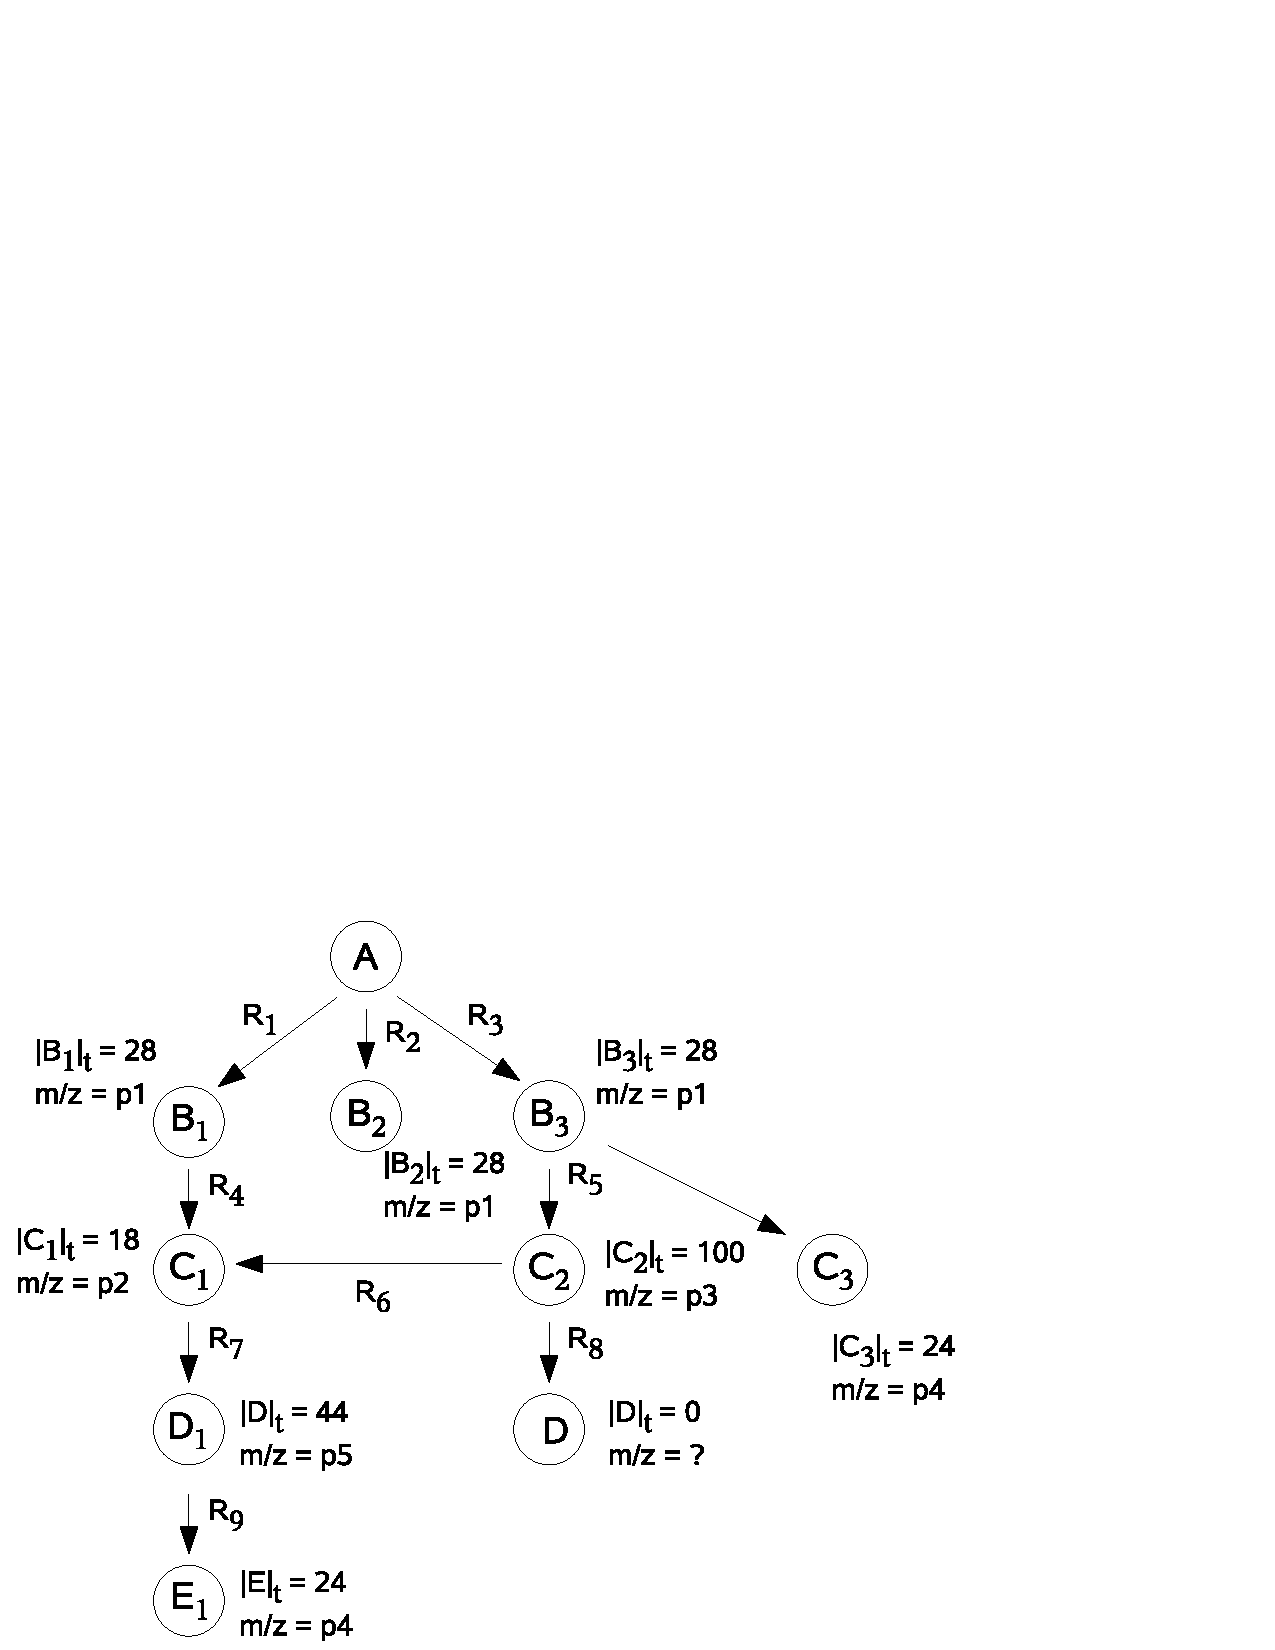
\includegraphics[scale=.8]{figures/exampleReaction.pdf} \caption[Example Calculating 
Probabilities]{{\bf{Example Calculating Probabilities}}.Example for the 
calculation of reaction probabilities from substance $A$. Each circle 
represents one different structure. $R_n$ defines the reaction process. $|A|_t$ 
is the frequency observed in the experimental mass spectrum. $p_n$ is the $m/z$ 
corresponding to the structure.}
  \label{fig:exampleReaction}
 \end{center}
\end{figure}

The Figure \ref{fig:exampleReaction} shows an example for the calculation of 
reaction probabilities. But in this case is drown a more complexer network than 
Schutz. It tries to represent all cases; obtaining more than 1 products, the 
same product for different reactions, symmetry of reactions. The $|X|$ is the 
concentration of the substance according the time. $t$ represents the time 
which the spectrum was obtained. sub-index $0$ represents the concentration in 
the time initial.



\begin{equation}
\label{p1}
P_1 = 1.0-\left( \frac{\left |A \right 
|_t}{\left|A\right|_0}\right)^{-\frac{\textstyle B_{j}}{\textstyle \sum_{k=1}^N 
B_{N}}} = 1.0-\left( \frac{20}{85.5}\right)^{\frac{\textstyle 20}{\textstyle 
60}} = 0.45
\end{equation}

\begin{equation}
\label{p2}
P_2 = 1.0-\left( \frac{20}{45}\right)^{\frac{\textstyle 25}{\textstyle 60}} = 
0.29
\end{equation}

\begin{equation}
\label{p3}
P_3 = 1.0-\left( \frac{20}{185.5}\right)^{\frac{\textstyle 10}{\textstyle 60}} 
= 0.31
\end{equation}


\begin{equation}
\label{p4}
P_4 = 1.0-\left( \frac{25}{65.5}\right)^{1} = 0.62
\end{equation}

\begin{equation}
\label{p5}
P_5 = 1.0- \frac{20}{150.5} = 0.93
\end{equation}


\begin{equation}
\label{p6}
P_6 = 1.0-\frac{15.5}{140.5} = 0.29
\end{equation}


\begin{equation}
\label{p7}
P_7 = 1.0-\frac{25}{40.5} = 0.69
\end{equation}


\begin{equation}
\label{p8}
P_0 = 0.0
\end{equation}

In the case of obtaining reactants which are not shown in the mass spectrum, 
they are defined as no reactive. Thus, their probability for us is 0. The 
definition is not completely correct because the reaction can happen but it 
reactant is too unstable with which reacts again. This makes that the reactant 
will not be shown in the mass spectrum.

\subsection{Output Results}

After the reaction generator has ended the evaluation of a sufficient quantity 
of compounds with their respective spectra stands to disposition fragmentation 
probabilities. This information will be used posteriorly by machine learning 
for the award of new fragmentations. Therefore it is necessary to store this 
information about the fragment and its probability value.


The reaction is not stored as such but it is stored by the results of different 
descriptors describing the reaction centre. Each reaction type has its 
specifies descriptors and the number of them and the file format chosen is the 
Attribute-Relation File Format (ARFF) used by Weka\cite{weka2005}. ARFF files have 
two distinct sections. The first section is the Header information, which is 
followed the Data information. In the figure X is shown an reaction example. In 
it is specified the results.



The relation declaration defines the name. All attributes declaration except 
one are numeric values. They are the descriptor calculation results. The class 
attribute contains in this case the classification of probabilities in this 
case segmented in 100 parts, from 0.0 to 1.0 with division of 0.01. And finally 
in the data declaration is put the instance. In the figure contains only one 
representing the reaction in Figure X. Thus each fragmentation reaction is 
defined as a instance.



    
%%%%%%%%%%%%%%%%%%%%%%%%%%%%%%%%
\section*{Authors contributions}
    Text for this section \ldots

    

%%%%%%%%%%%%%%%%%%%%%%%%%%%
\section*{Acknowledgements}
  \ifthenelse{\boolean{publ}}{\small}{}
  Text for this section \ldots


 
%%%%%%%%%%%%%%%%%%%%%%%%%%%%%%%%%%%%%%%%%%%%%%%%%%%%%%%%%%%%%
%%                  The Bibliography                       %%
%%                                                         %%              
%%  Bmc_article.bst  will be used to                       %%
%%  create a .BBL file for submission, which includes      %%
%%  XML structured for BMC.                                %%
%%  After submission of the .TEX file,                     %%
%%  you will be prompted to submit your .BBL file.         %%
%%                                                         %%
%%                                                         %%
%%  Note that the displayed Bibliography will not          %% 
%%  necessarily be rendered by Latex exactly as specified  %%
%%  in the online Instructions for Authors.                %% 
%%                                                         %%
%%%%%%%%%%%%%%%%%%%%%%%%%%%%%%%%%%%%%%%%%%%%%%%%%%%%%%%%%%%%%


{\ifthenelse{\boolean{publ}}{\footnotesize}{\small}
 \bibliographystyle{bmc_article}  % Style BST file
  \bibliography{bmc_article} }     % Bibliography file (usually '*.bib' ) 

%%%%%%%%%%%

\ifthenelse{\boolean{publ}}{\end{multicols}}{}

%%%%%%%%%%%%%%%%%%%%%%%%%%%%%%%%%%%
%%                               %%
%% Figures                       %%
%%                               %%
%% NB: this is for captions and  %%
%% Titles. All graphics must be  %%
%% submitted separately and NOT  %%
%% included in the Tex document  %%
%%                               %%
%%%%%%%%%%%%%%%%%%%%%%%%%%%%%%%%%%%

%%
%% Do not use \listoffigures as most will included as separate files

\section*{Figures}
  \subsection*{The evaluation storage of a fragmentation 
reaction in the database. The database consists of ARFF files. The reaction is 
described by strategic descriptors.}

\subsection*{Figure 2 - Sample figure title}
      Figure legend text.



%%%%%%%%%%%%%%%%%%%%%%%%%%%%%%%%%%%
%%                               %%
%% Tables                        %%
%%                               %%
%%%%%%%%%%%%%%%%%%%%%%%%%%%%%%%%%%%

%% Use of \listoftables is discouraged.
%%
\section*{Tables}
  \subsection*{Table 1 - Sample table title}
    Here is an example of a \emph{small} table in \LaTeX\ using  
    \verb|\tabular{...}|. This is where the description of the table 
    should go. \par \mbox{}
    \par
    \mbox{
      \begin{tabular}{|c|c|c|}
        \hline \multicolumn{3}{|c|}{My Table}\\ \hline
        A1 & B2  & C3 \\ \hline
        A2 & ... & .. \\ \hline
        A3 & ..  & .  \\ \hline
      \end{tabular}
      }
  \subsection*{Table 2 - Sample table title}
    Large tables are attached as separate files but should
    still be described here.



%%%%%%%%%%%%%%%%%%%%%%%%%%%%%%%%%%%
%%                               %%
%% Additional Files              %%
%%                               %%
%%%%%%%%%%%%%%%%%%%%%%%%%%%%%%%%%%%

\section*{Additional Files}
  \subsection*{Additional file 1 --- Sample additional file title}
    Additional file descriptions text (including details of how to
    view the file, if it is in a non-standard format or the file extension).  This might
    refer to a multi-page table or a figure.

  \subsection*{Additional file 2 --- Sample additional file title}
    Additional file descriptions text.


\end{bmcformat}
\end{document}







